\documentclass{article}

\usepackage{graphicx}
\usepackage{tikz}
\usepackage{tikzsymbols}
\usetikzlibrary{calc,patterns,shapes.geometric}
\pagestyle{empty}
\usepackage[margin=0pt]{geometry}
\geometry{papersize={14in,12in}}

\def\centerarc[#1](#2)(#3:#4:#5){\draw[#1] ($(#2)+({#5*cos(#3)},{#5*sin(#3)})$) arc (#3:#4:#5);}

\begin{document}
	\begin{figure}
		\centering
		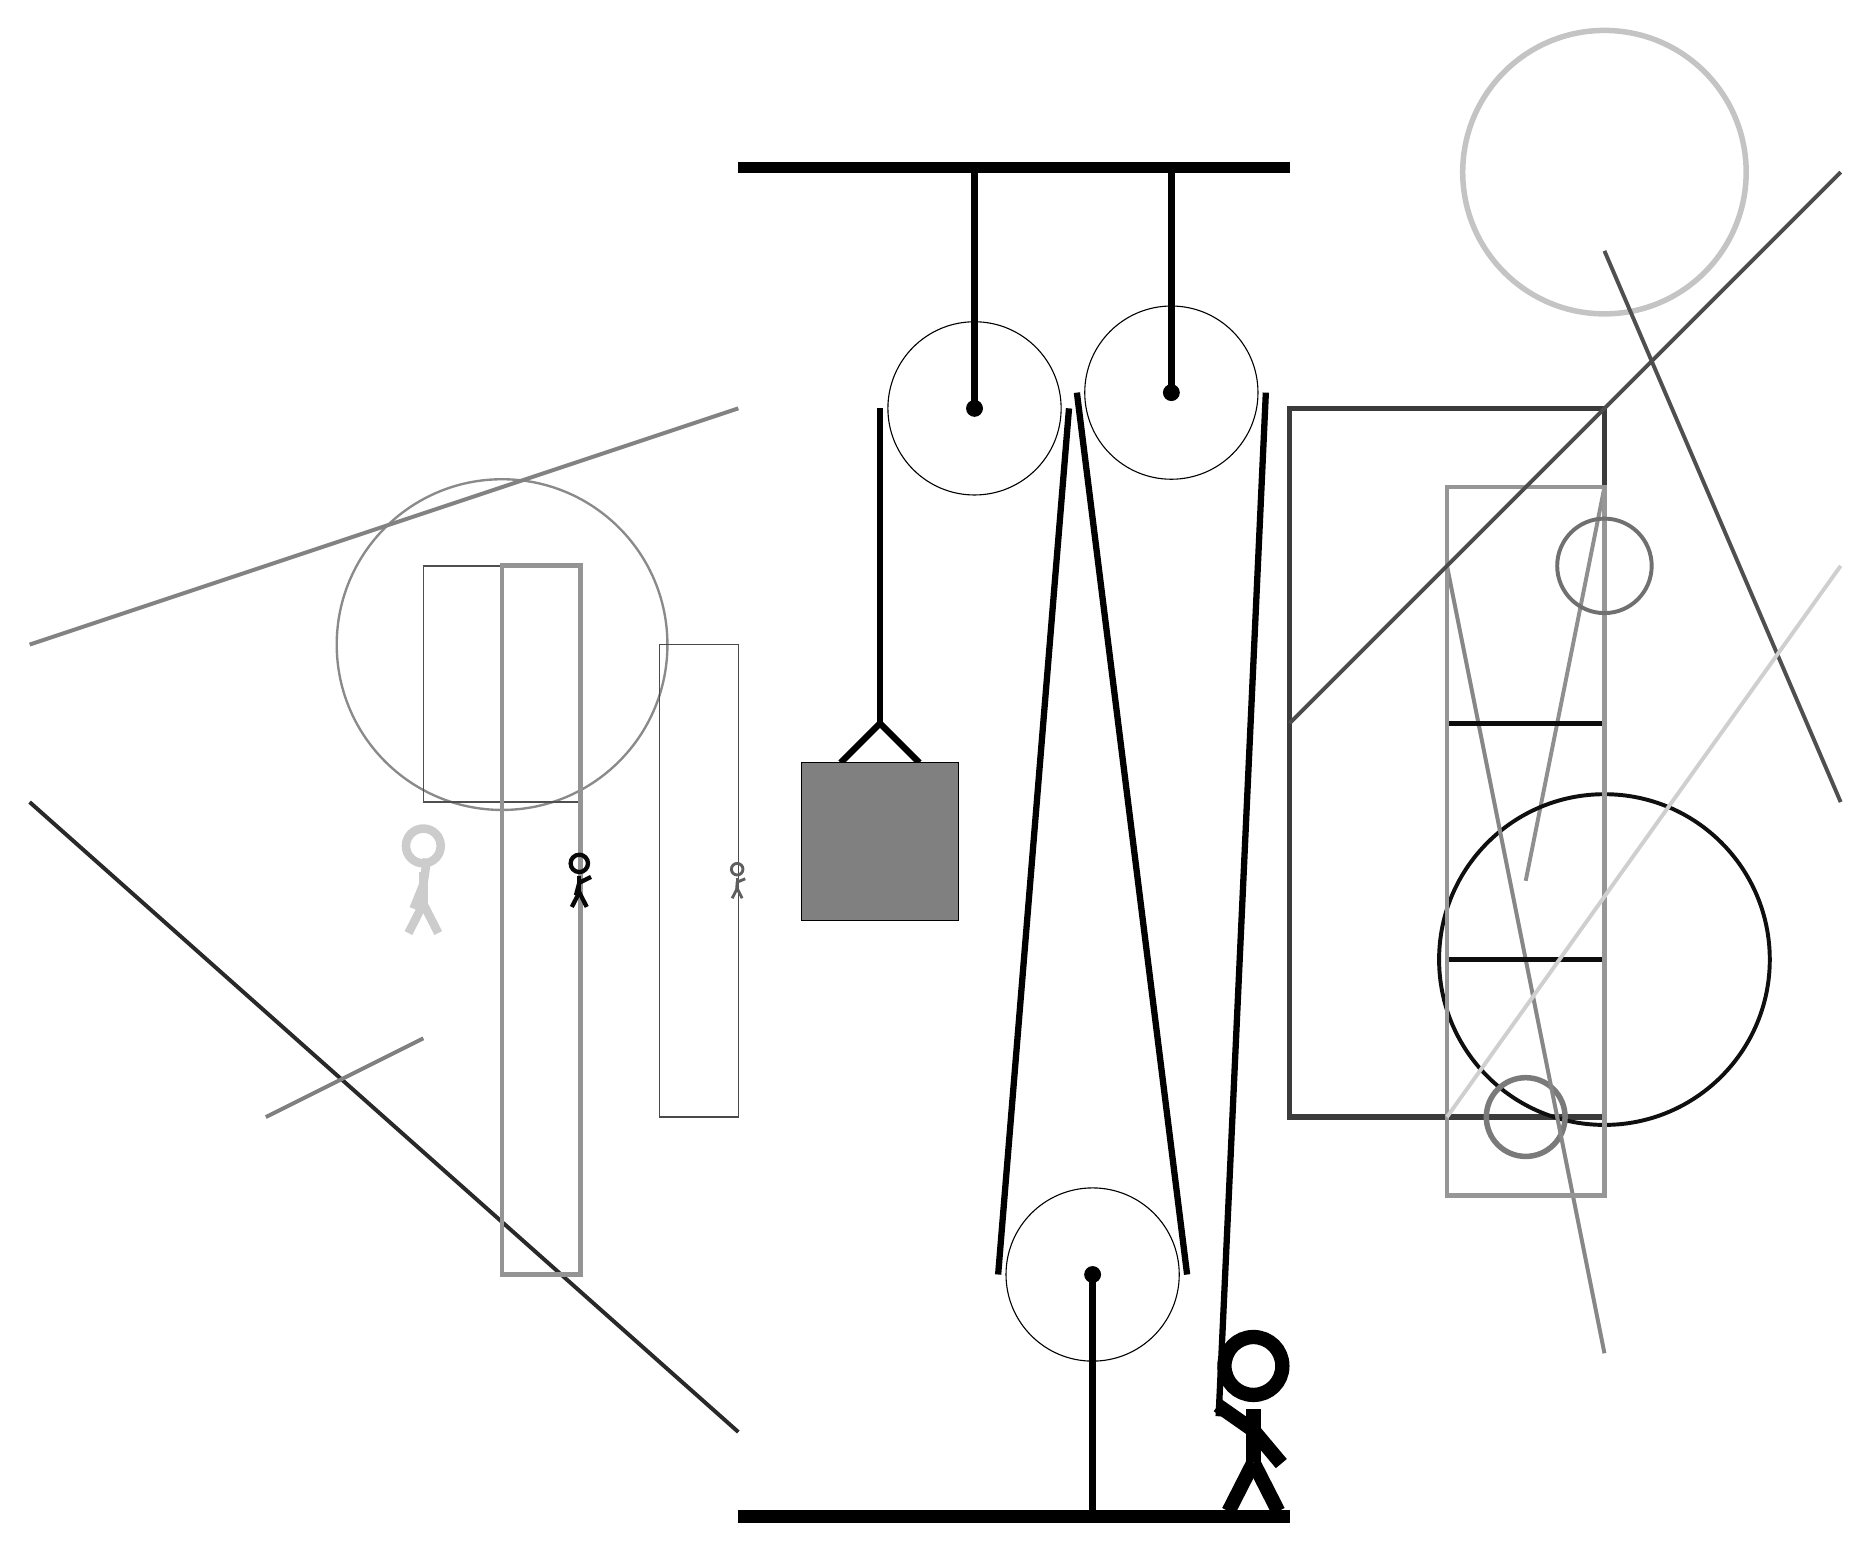
\begin{tikzpicture}
			%%%%% START %%%%%
			
			\draw[fill=black] (-2, 14) rectangle (5, 14.125);
			
			\draw (1, 11) circle (1.1);
			\draw[fill=black] (1, 11) circle (0.1);
			\draw[line width=0.8mm]  (1, 14) -- (1, 11);
			
			\draw[fill=white](2.5, 0) circle (1.1);
			\draw[fill=black] (2.5, 0) circle (0.1);
			\draw[line width=0.8mm]  (2.5, -3) -- (2.5, 0);
			
			\draw[fill=white](3.5, 11.2) circle (1.1);
			\draw[fill=black] (3.5, 11.2) circle (0.1);
			\draw[line width=0.8mm] (3.5, 14) -- (3.5, 11.2);
			
			\draw[line width=0.8mm] (-0.7, 6.5) -- (-0.2, 7.0) -- (0.3, 6.5);
			\draw[fill=black!50] (-1.2, 6.5) rectangle (0.8, 4.5);
			
			\draw[line width=0.8mm] (-0.2, 11) -- (-0.2, 7.0);
			\centerarc[line width=0.8mm](1, 11)(0:180:1.2000000000000002);
			\draw[line width=0.8mm](2.2, 11) -- (1.3, 0);
			\centerarc[line width=0.8mm](2.5, 0)(180:360:1.2000000000000002);
			\draw[line width=0.8mm](3.7, 0) -- (2.3, 11.2);
			\centerarc[line width=0.8mm](3.5, 11.2)(0:180:1.2000000000000002);
			\draw[line width=0.8mm](4.7, 11.2) -- (4.1, -1.8);
			
			\node at (4.5, -1.9) {\Strichmaxerl[10][-35][-50]};
			
			\draw[line width=0.5mm, color=black!44](8, 5) -- (9, 10);
			
			\draw[line width=0.7mm, color=black!77] (5, 2) rectangle (9, 11);
			\node[line width=0.3mm, color=black!20] at (-6, 5) {\Strichmaxerl[6][68][82]};
			\draw [line width=0.5mm, color=black!94](9, 4) circle (2.1);
			\draw [line width=0.7mm, color=black!52](8, 2) circle (0.5);
			
			\draw[line width=0.5mm, color=black!47](7, 9) -- (9, -1);
			
			\draw[line width=0.6mm, color=black!95] (7, 4) rectangle (9, 7);
			\draw [line width=0.7mm, color=black!23](9, 14) circle (1.8);
			\draw [line width=0.3mm, color=black!46](-5, 8) circle (2.1);
			
			\draw[line width=0.5mm, color=black!69](9, 13) -- (12, 6);
			
			\draw[line width=0.2mm, color=black!71] (-2, 8) rectangle (-3, 2);
			
			\draw[line width=0.2mm, color=black!69] (-4, 9) rectangle (-6, 6);
			\draw[line width=0.5mm, color=black!49](-2, 11) -- (-11, 8);
			
			\node[line width=0.4mm, color=black!63] at (-2, 5) {\Strichmaxerl[2][86][22]};
			\draw[line width=0.5mm, color=black!84](-2, -2) -- (-11, 6);
			\draw[line width=0.6mm, color=black!41] (7, 10) rectangle (9, 1);
			\draw[line width=0.5mm, color=black!70](5, 7) -- (12, 14);
			
			\draw[line width=0.5mm, color=black!19](7, 2) -- (12, 9);
			\draw [line width=0.5mm, color=black!56](9, 9) circle (0.6);
			\draw[line width=0.6mm, color=black!42] (-4, 9) rectangle (-5, 0);
			\draw[line width=0.5mm, color=black!50](-6, 3) -- (-8, 2);
			
			\node[line width=0.6mm, color=black!97] at (-4, 5) {\Strichmaxerl[3][75][26]};
			
			\draw[fill=black] (-2, -3) rectangle (5, -3.15);
			
			%%%%% END %%%%%
		\end{tikzpicture}
	\end{figure}	
\end{document}